
\subsection{Comparison to Other High-Redshift Measurements}

In Figure~\ref{fig:ratecompilation} we compare our results to an
assortment of other volumetric SN Ia rate measurements. (Most
published measurements use the same cosmology used here; those that do
not have been corrected to our assumed cosmology.) At $z \gtrsim 1$
the three existing measurements are \citet[][hereafter
  Ku08]{kuznetsova08a}, \citet[][hereafter D08]{dahlen08a}, and
\citet[][hereafter G11]{graur11a}. D08 and G11 supplant earlier
results from \citet{dahlen04a} and \citet{poznanski07a},
respectively. The Ku08 and D08 measurements are based on SN searches
in the \emph{HST} GOODS fields, with Ku08 being an independent
analysis of a subset of the data used in D08. These SN searches used
ACS to cover the GOODS fields with a 45 day cadence and triggered
followup (imaging and spectroscopy) of SN candidates. The D08 analysis
uses a SN typing method based on both spectroscopy and photometry
(similar to the approach used here) while Ku08 use a photometric-only
pseudo-Bayesian approach to typing. The G11 measurement is based on
``single-detection'' searches in the Subaru Deep Field. G11 also use a
pseudo-Bayesian typing approach, but use a single detection with
observations in three filters, rather than multiple detections with
observation in (typically) two filters as in Ku08.

\begin{figure}[tb]
\begin{center}
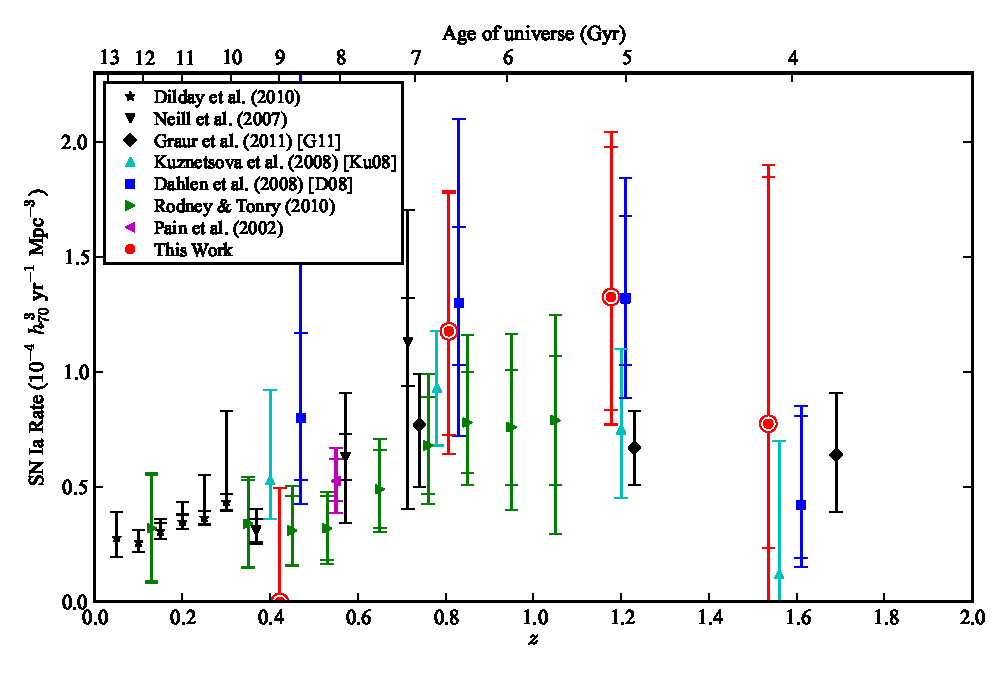
\includegraphics[width=\textwidth]{figures/fieldrate/ratecompilation.eps}
\end{center}
\caption[Volumetric SN~Ia rates from this work and the
  literature]{Volumetric SN~Ia rates from the \emph{HST} Cluster
  Supernova Survey (red points) compared to key rates from the
  literature. For measurements with two error bars, including ours,
  the inner and outer error bars represent the statistical (Poisson)
  and total (statistical + systematic) uncertainties,
  respectively. Measurements with a single error bar (Ku08 and G11)
  are Bayesian-based analyses where the error bar encompasses both
  statistical and typing uncertainties.\label{fig:ratecompilation}}
\end{figure}

Our results in the three highest redshift bins are very similar to D08
and are consistent with G11 and Ku08 at the $\sim$$1\sigma$
level. Even with limited statistics of only $\sim$12 SNe~Ia, they
provide additional strong evidence that the SN rate is $\gtrsim 0.6
\times 10^{-4}$~$h_{70}^{3}$~yr$^{-1}$~Mpc$^{-3}$ at $z \sim 1$. With
the data available from Figure~\ref{fig:ctarea1} and the SN candidate
list, the rates from this survey can be recomputed in any arbitrary
bin and for a variety of assumptions about SN properties and host
galaxy dust distributions. This will make it easy to combine these
results with other measurements for increased statistical power.

\subsection{Comparison of Host-Galaxy Dust Distributions}

In light of the large systematic differences noted
in \S\ref{sec:sysdust} due to choice of host galaxy dust distribution,
it is interesting to compare the distributions used in D08, Ku08 and
G11.  

For their main result, D08 use a distribution similar to model A used
here, and also consider models similar to B and C. (Our models A, B
and C are based on models with the same labels in D08.) If we had
assumed model A, our derived rates in the two mid-redshift bins
would have been $\sim$$30\%$ higher, implying rates larger than
those found in D08. Interestingly, D08 do not find the large
difference between model A and models B/C that we find here. They find
that model B produces rates that are $\lesssim 10\%$ lower than model
A (only $\sim$$4\%$ in the highest redshift bin). Model C is found to
have even less of an effect (and actually \emph{increases} rates
relative to model A in the highest bin). It is difficult to know
whether this difference could be due to the different cadence
($\sim$23~days here versus $\sim$45~days in GOODS), difference in
details of the efficiency simulations, or some other cause.

Both Ku08 and G11 use distributions lacking the high-extinction tail
of model A and are thus more similar to models B/C or K09. Ku08 use
only two discrete values, $A_V = 0.0$ and 0.4 (but also consider the
case $A_V = 1.0$ in assessing systematic uncertainty). G11 use the
distribution of N06 (model C), but truncated at $A_V = 1$ (eliminating
the highest-extinction $\sim$$10\%$ of the distribution). In contrast,
40\% of SNe have $A_V > 1$ in model A. This difference in assumptions
might explain some differences in the results. In particular, it would
explain why the D08 result is much higher than K08 despite the large
overlap in datasets. It would also partially explain why the D08
result is significantly higher than the G11 result in the $0.6 < z <
1.4$ redshift range. 
